% ============================================================
%  FedMKS --- IEEE Conference Paper
%  Compile: pdflatex paper.tex
%  Requires: IEEEtran, tikz, pgfplots, pgfplotsgroup, graphicx,
%            fontawesome5, algorithm, algpseudocode
% ============================================================
\documentclass[conference]{IEEEtran}
\usepackage{graphicx}
\usepackage{tikz}
\usepackage{pgfplots}
\pgfplotsset{compat=1.18}
\usepgfplotslibrary{groupplots}
\usepackage{amsmath,amssymb}
\usepackage{booktabs}
\usepackage{tabularx}
\usepackage{multirow}
\usepackage{array}
\usepackage{xcolor}
\usepackage{microtype}
\usepackage{fontawesome5}
\usepackage{algorithm}
\usepackage{algpseudocode}
\usepackage{url}
\usepackage{cite}
\usetikzlibrary{arrows.meta,shapes,positioning,fit,
                decorations.pathreplacing,calc,backgrounds}

% ── Palette ──────────────────────────────────────────────────────────────────
\definecolor{clBlue}  {RGB}{52,120,180}
\definecolor{clGreen} {RGB}{45,155,75}
\definecolor{clOrange}{RGB}{210,105,30}
\definecolor{clPurple}{RGB}{120,55,175}
\definecolor{clGray}  {RGB}{100,100,100}
\definecolor{clTeal}  {RGB}{0,130,115}
\definecolor{clRed}   {RGB}{185,0,0}
\definecolor{clOlive} {RGB}{100,100,0}
\definecolor{ltBlue}  {RGB}{220,234,252}
\definecolor{ltGreen} {RGB}{215,244,220}
\definecolor{ltOrange}{RGB}{255,237,212}
\definecolor{ltYellow}{RGB}{255,251,212}
\definecolor{ltPurple}{RGB}{238,225,255}
\definecolor{ltGray}  {RGB}{238,238,238}
\definecolor{ltRed}   {RGB}{255,220,220}

% ── TikZ shared styles ───────────────────────────────────────────────────────
\tikzset{
  blk/.style={rectangle,draw=black!35,rounded corners=2pt,
              minimum height=0.50cm,align=center,
              font=\scriptsize,line width=0.4pt},
  pipe/.style={rectangle,draw=black!35,rounded corners=2pt,
               minimum height=0.50cm,minimum width=1.55cm,align=center,
               font=\scriptsize,line width=0.42pt},
  arr/.style={-{Stealth[length=2.8pt,width=1.9pt]},semithick},
}

% ── pgfplots panel style ─────────────────────────────────────────────
\pgfplotsset{
  p1panel/.style={
    width=0.465\textwidth,
    height=3.0cm,
    grid=major,
    grid style={gray!18, line width=0.3pt},
    tick label style={font=\tiny},
    label style={font=\tiny},
    title style={font=\scriptsize\bfseries},
    xlabel={Round},
    ylabel={Val.\ Acc.\ (\%)},
    xtick={10,20,30,40,50},
    xmin=0,xmax=52,
    tick pos=left,
    line width=0.65pt,
    enlarge x limits=0.02,
  }
}

% ============================================================
\title{FedMKS: A Hybrid Model and Knowledge Sharing Approach\\
  for Robust Federated Learning in Heterogeneous Networks}

\author{%
  \IEEEauthorblockN{Gad Gad\IEEEauthorrefmark{1},
    Mostafa Fouda\IEEEauthorrefmark{2},
    Zubair Md Fadlullah\IEEEauthorrefmark{1}}
  \IEEEauthorblockA{\IEEEauthorrefmark{1}Department of Computer Science,
    Western University, London, ON, Canada}
  \IEEEauthorblockA{\IEEEauthorrefmark{2}Department of Electrical and
    Computer Engineering, Idaho State University, Pocatello, ID, USA}
  \IEEEauthorblockA{Emails: ggad@uwo.ca, mfouda@ieee.org,
    zfadlullah@ieee.org}
}
% ============================================================

\begin{document}
\maketitle

% ─────────────────────────────────────────────────────────────────────────────
\begin{abstract}
Federated Learning (FL) enables distributed clients to train a shared
model without exchanging raw data, making it attractive for
privacy-sensitive edge applications.  Real deployments, however, face
\emph{system heterogeneity}: devices differ widely in compute capability,
so no single model architecture fits all clients.
Knowledge-distillation-based FL sidesteps this constraint by exchanging
soft labels on a shared public set instead of weights, allowing each
client to keep its own architecture.  Yet under \emph{statistical
heterogeneity} (non-IID label skew), soft-label-only distillation
degrades sharply and can underperform simple weight averaging on a
common small model.  We present \textbf{FedMKS} (Federated Learning
with Model and Knowledge Sharing), a hybrid algorithm that organises
clients into architecture tiers and couples intra-tier weight averaging
with cross-tier soft-label distillation, recovering the accuracy of
weight sharing while preserving architectural diversity.  We apply
FedMKS to indoor Wi-Fi CSI sensing for occupancy and activity
detection---a privacy-critical setting where raw data cannot leave the
home---and evaluate it on the HomeOccupancy CSI dataset and
MNIST/CIFAR-10 under IID and non-IID partitions against FedMD, FedAKD,
FedAvg, FedProx, FedDF, and Local/Centralised baselines.  FedMKS attains
90.4\% on HomeOccupancy IID---within 0.5\% of the centralised ceiling.
Code and datasets are publicly available.
\end{abstract}

% ─────────────────────────────────────────────────────────────────────────────
\section{Introduction}
\label{sec:intro}

Federated Learning (FL) allows a population of edge devices to
collaboratively train a model while keeping raw data on
device~\cite{mcmahan2017fedavg}.  This privacy-preserving paradigm is
appealing wherever data is sensitive, scarce, or expensive to
centralise---smart homes, healthcare, and mobile sensing being canonical
examples.

A persistent obstacle is \emph{system heterogeneity}: edge devices range
from constrained sensors to capable gateways, so no single architecture
fits all.  Weight-sharing methods (FedAvg, FedProx) require identical
architectures and therefore force every client onto the smallest common
model.  Knowledge-distillation methods (FedMD, FedAKD, FedDF) remove this
constraint by exchanging soft labels on a shared public set rather than
weights, letting each client keep an architecture matched to its
hardware.

Distillation alone, however, suffers under \emph{statistical
heterogeneity}: when client label distributions are non-IID, soft-label
averaging provides a weaker training signal than weight averaging, and
our experiments show KD-only methods trailing even all-small weight
sharing by double-digit margins.  This motivates a \emph{hybrid}
architecture that combines both channels---averaging weights where
architectures match and distilling soft labels where they do not.

We instantiate this idea for indoor Wi-Fi sensing: Channel State
Information (CSI) encodes fine-grained multipath propagation effects that
shift when a person moves, breathes, or changes posture, enabling
camera-free occupancy and activity recognition from commodity access
points~\cite{ma2019survey, yousefi2017survey}.  Labelled CSI is private
and hard to collect at scale, making it a natural application for
heterogeneous FL.

\textbf{Contribution.}  We propose \textbf{FedMKS} (Federated Learning
with Model and Knowledge Sharing), which (i)~partitions clients into
architecture tiers and shares classifier weights within each tier,
(ii)~shares distilled soft labels across tiers on a public set, and
(iii)~applies Mixup augmentation before distillation.  A dual-head tiered
model decouples private classification from public-set distillation, so
clients of different capacity collaborate without exchanging raw data.

\begin{figure*}[t]
\centering
\begin{minipage}[t]{0.495\textwidth}
  \centering
  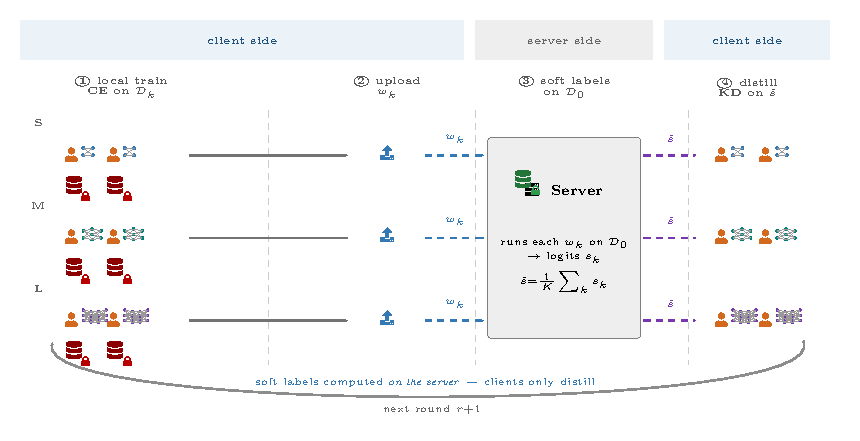
\includegraphics[width=\linewidth]{assets/feddf_v2.pdf}\\[1pt]
  {\footnotesize (a)~FedDF~\cite{lin2020ensemble}: soft labels computed
   \emph{on the server}.}
\end{minipage}\hfill
\begin{minipage}[t]{0.495\textwidth}
  \centering
  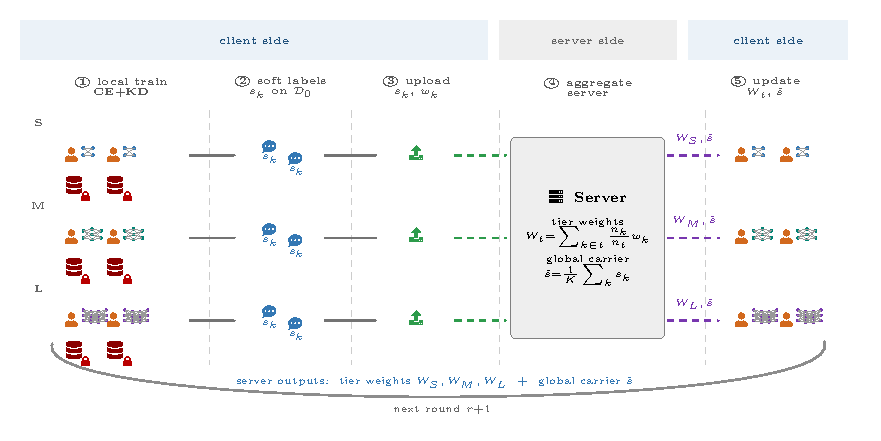
\includegraphics[width=\linewidth]{assets/fedmks_v2.pdf}\\[1pt]
  {\footnotesize (b)~FedMKS (ours): soft labels computed \emph{on each
   client}; server also averages intra-tier weights.}
\end{minipage}
\caption{\textbf{FedDF vs.\ FedMKS --- one communication round.}
  FedDF uploads client weights and runs every model on the public set at
  the server; FedMKS computes soft labels $s_k$ on each client, so the
  server only averages tensors and additionally FedAvgs intra-tier
  weights ($W_S,W_M,W_L$).}
\label{fig:fedmksoverview}
\end{figure*}

% ─────────────────────────────────────────────────────────────────────────────
\section{Related Work}
\label{sec:related}

Figure~\ref{fig:fltimeline} sketches the FL research timeline relevant
to this work; we review federated learning in general, distillation-based
FL for system heterogeneity, the impact of statistical heterogeneity, and
Wi-Fi sensing as our target application.

\begin{figure*}[t]
\centering
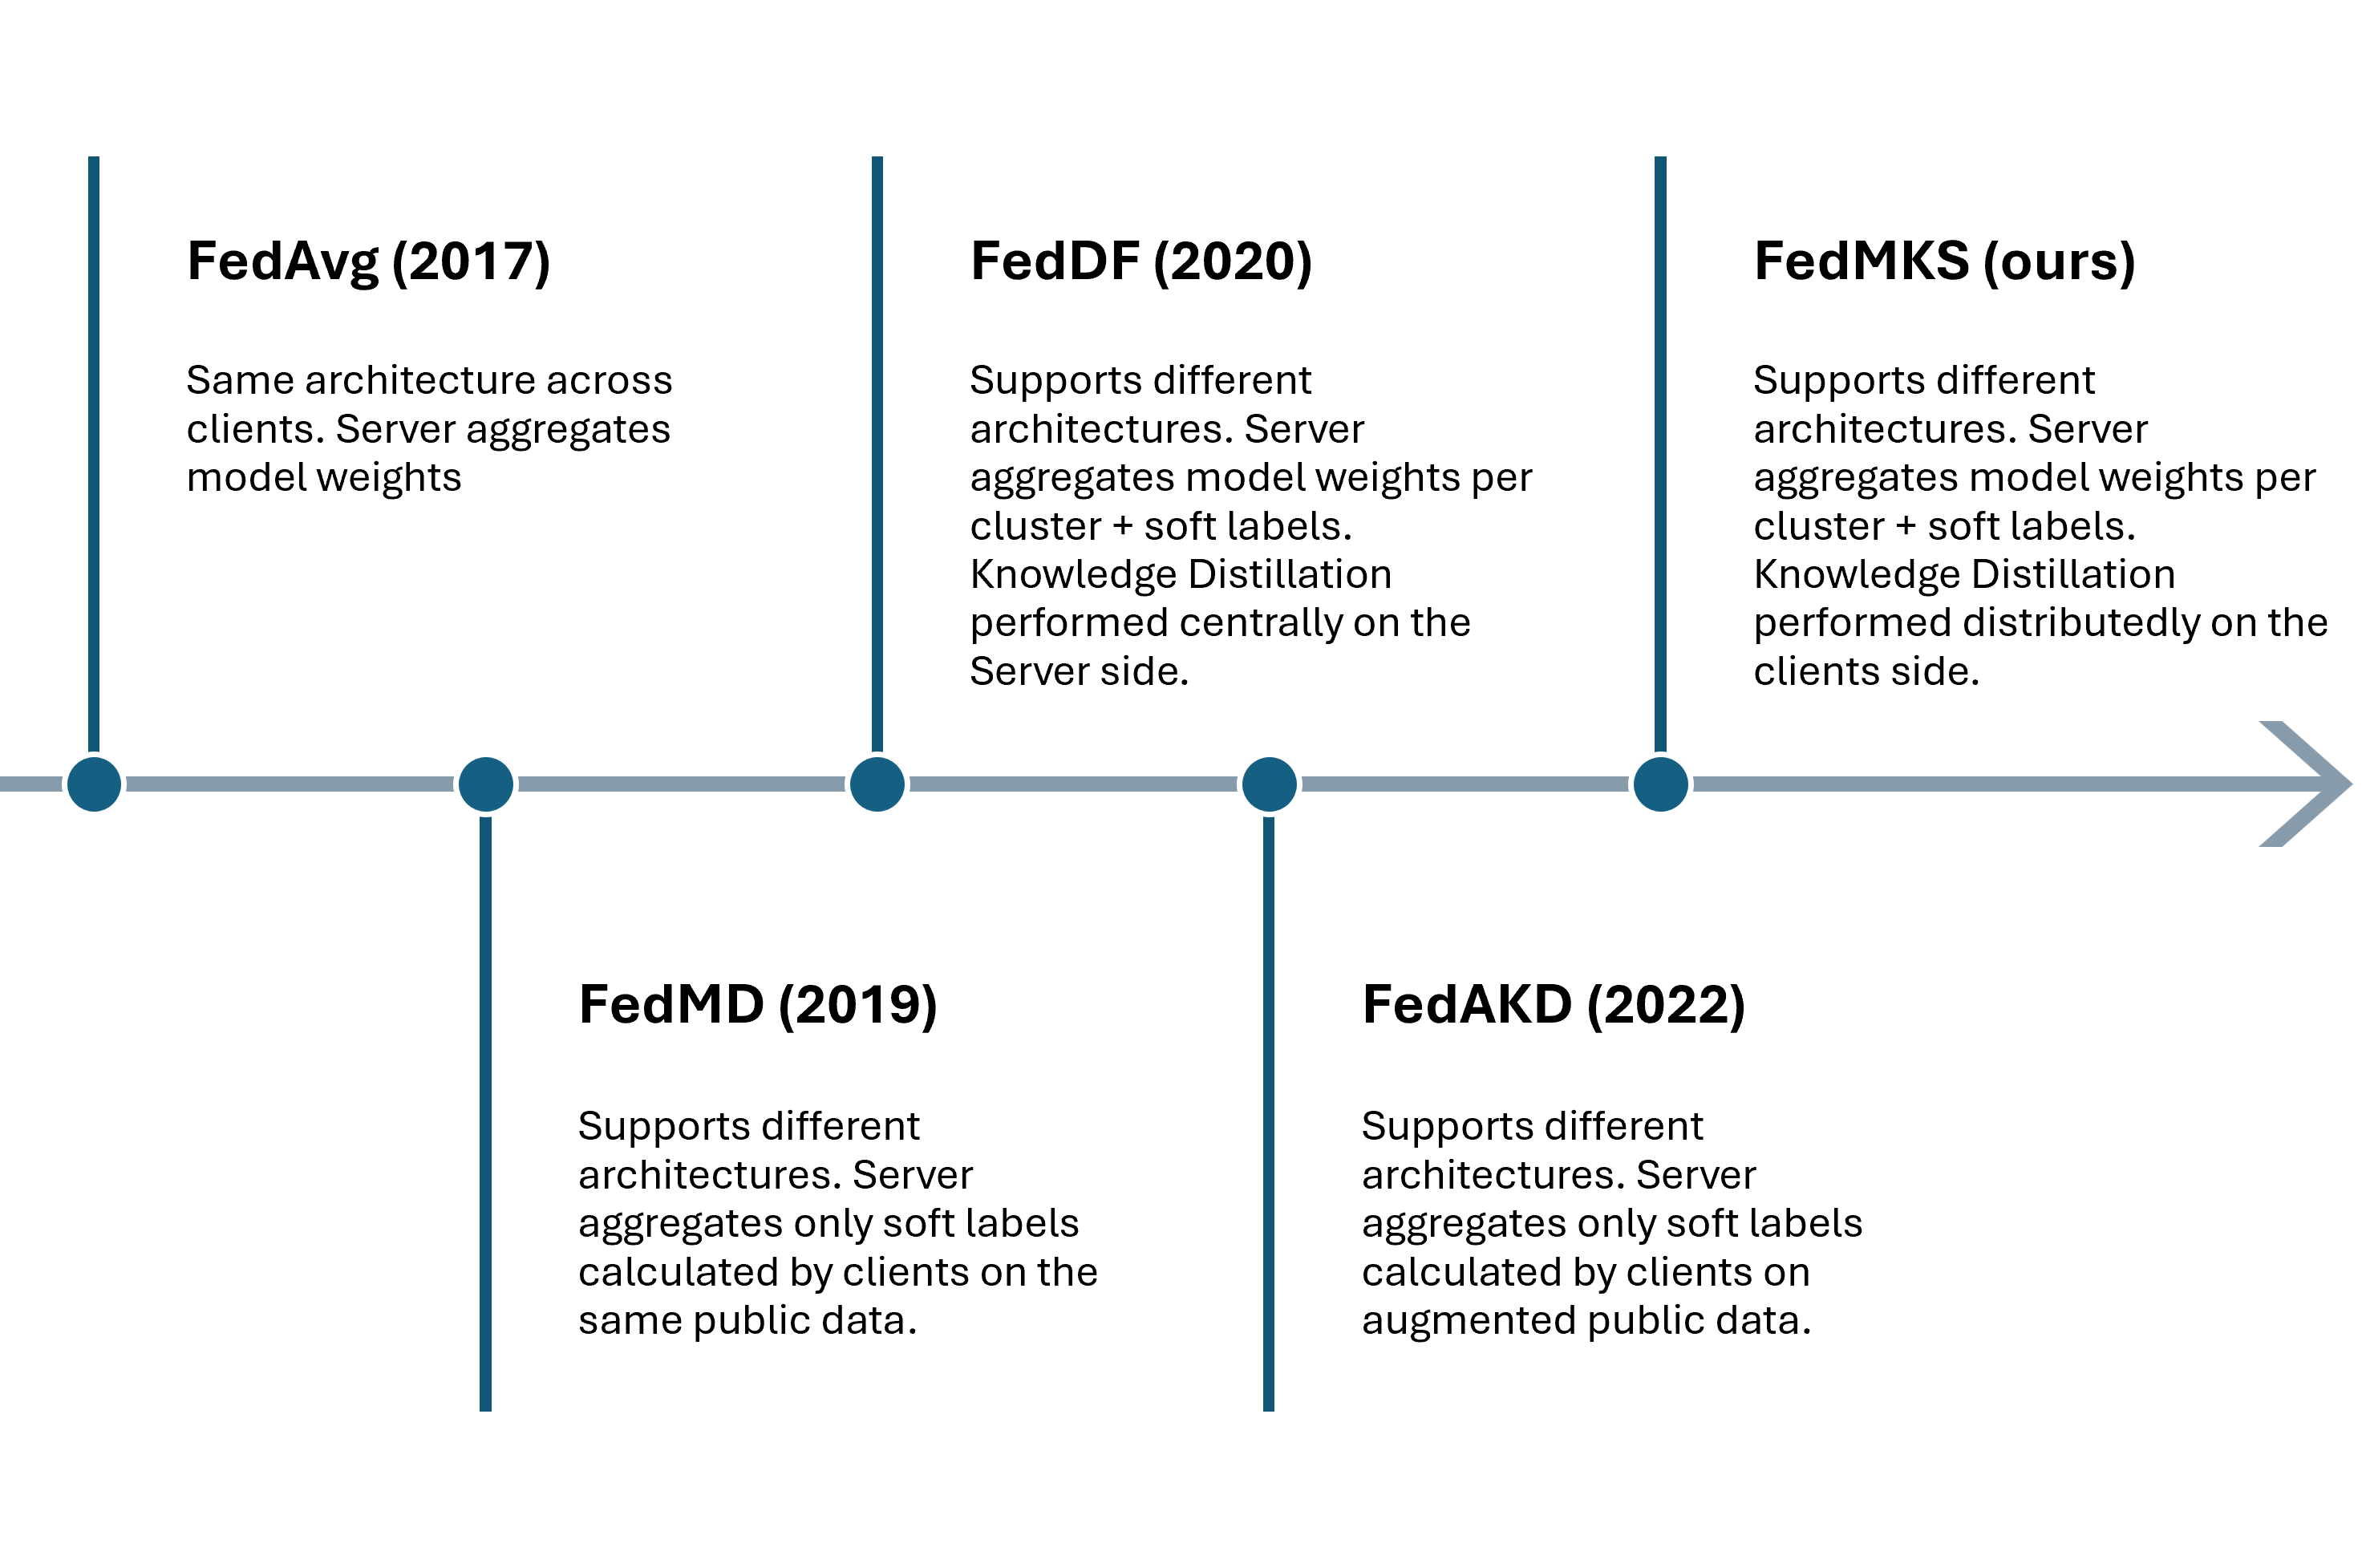
\includegraphics[width=0.52\textwidth]{assets/FL_literature.png}
\caption{Timeline of federated-learning research relevant to this work.}
\label{fig:fltimeline}
\end{figure*}

\subsection{Federated Learning}

FedAvg~\cite{mcmahan2017fedavg} introduced federated averaging of
locally trained weights and remains the canonical FL baseline, but it
requires identical architectures across clients;
FedProx~\cite{li2020fedprox} adds a proximal term that tolerates
statistical and system heterogeneity while keeping the same
architectural constraint.  Sozinov~et~al.~\cite{sozinov2018fedhar}
first showed federated HAR can rival centralised accuracy while
preserving privacy; Wu~et~al.~\cite{wu2021fedcsi} extended FL to CSI
sensing, where non-IID per-home distributions degrade FedAvg and
motivate personalised
approaches~\cite{ek2020fedwifi,ouyang2021clusterfl,presotto2022semfed}.

\subsection{Knowledge-Distillation-Based FL}

FedMD~\cite{li2019fedmd} removes the architecture constraint by sharing
only soft predictions on a public set, building on Hinton's distillation
framework~\cite{hinton2015distill}; federated mutual
learning~\cite{shen2020fedml} distils peer-to-peer.
FedDF~\cite{lin2020ensemble} instead ensembles client models on the
server and distils a fused student centrally.  Unlike FedDF, FedMKS
distributes distillation across clients, removing the server bottleneck
at the cost of higher client workload.

\subsection{Statistical Heterogeneity}

Zhao~et~al.~\cite{zhao2018noniid} quantify the sharp accuracy drop of
FL under non-IID data.  Weight averaging suffers from client drift,
while soft-label distillation provides a weaker per-round signal; our
results confirm that KD-only methods degrade more severely under label
skew than weight-sharing methods, motivating hybrid designs that combine
both channels.

\subsection{Wi-Fi Sensing}

Wi-Fi CSI sensing has progressed from coarse localisation to fine-grained
activity and gesture recognition~\cite{ma2019survey,yousefi2017survey}.
Early systems showed that commodity 802.11 reflections encode human
presence and activities~\cite{adib2013seewall,wang2014eyes}; later work
added real-time gesture classification~\cite{chen2018gesture},
healthcare HAR~\cite{han2020healthcare}, environment
robustness~\cite{jiang2021envind}, and joint
localisation--recognition~\cite{liu2020deepmtd}.  Indoor occupancy
detection is a representative privacy-critical application: raw CSI
reveals presence and behaviour inside a home and cannot be centralised,
making it a natural fit for heterogeneous FL.

% ─────────────────────────────────────────────────────────────────────────────
\section{System Model}
\label{sec:sysmodel}

\subsection{Notation}

\begin{table}[t]
\centering\footnotesize
\caption{Symbol table.}
\label{tab:symbols}
\setlength{\tabcolsep}{4pt}
\begin{tabular}{@{}cl@{}}
\toprule
\textbf{Symbol} & \textbf{Meaning}\\
\midrule
$K$                          & Number of clients ($K{=}20$)\\
$\mathcal{K}$                & Client index set $\{1,\ldots,K\}$\\
$R$                          & Number of FL communication rounds ($R{=}50$)\\
$r$                          & Round index, $r\!\in\!\{1,\ldots,R\}$\\
$\mathcal{D}_k$              & Private labelled dataset of client $k$\\
$n_k$                        & $|\mathcal{D}_k|$; $n = \sum_k n_k$\\
$\mathcal{Y}$                & Global label space; $C{=}|\mathcal{Y}|$\\
$\mathcal{Y}_k$              & Local label subset, $\mathcal{Y}_k \subseteq \mathcal{Y}$\\
$\mathcal{D}^{\text{pub}}$   & Shared public (unlabelled) dataset\\
$t_k$                        & Tier of client $k$: S, M, or L\\
$\theta_k$                   & All trainable parameters of model $f_k$\\
$\theta_k^{\text{bb}}$       & Backbone parameters (shared by both heads)\\
$\mathbf{W}_t^{(r)}$         & Server-side averaged classifier weights for tier $t$ at round $r$\\
$d$                          & Distillation-head output dimension (soft-label size)\\
$s_k^{(r)}$                  & Soft-label matrix from client $k$ at round $r$,
                               $s_k^{(r)}\!\in\!\mathbb{R}^{|\mathcal{D}^{\text{pub}}|\times d}$\\
$\bar{s}^{(r)}$              & Aggregated global soft labels at round $r$\\
$T,B$                        & CSI window length ($1500$) and STFT bins ($8$)\\
\bottomrule
\end{tabular}
\end{table}

\subsection{Network and Data Model}

Consider a star-topology FL network with a central server and
$K{=}20$ clients.  Each client $k$ holds a private labelled dataset
$\mathcal{D}_k = \{(x_i^k, y_i^k)\}_{i=1}^{n_k}$,
where $x_i^k \in \mathbb{R}^{T \times (4+B)}$ is a preprocessed CSI window
and $y_i^k \in \mathcal{Y}_k \subseteq \mathcal{Y}$ its activity label.
Under \emph{IID} partitioning each client receives $n_c{=}30$ examples per
class; under \emph{non-IID}, class proportions follow
$\mathrm{Dir}(\alpha{=}0.5)$.  All clients also share an unlabelled
\emph{public} dataset $\mathcal{D}^{\text{pub}}$ (e.g.\ HomeHAR) used
exclusively for knowledge transfer.

\subsection{Heterogeneous Model Architecture}

Each client is assigned a compute tier
$t_k \in \{\text{S}, \text{M}, \text{L}\}$ reflecting its hardware budget.
Every tier instantiates a \emph{dual-head} model
$f_k = (\phi_k,\, h_k^{\text{clf}},\, h_k^{\text{dist}})$,
where $\phi_k$ is a shared backbone parameterised by
$\theta_k^{\text{bb}}$ and the two heads are trained with decoupled losses:

\begin{itemize}
  \item \textbf{Classification head} $h_k^{\text{clf}}$: trained on private
    data with cross-entropy loss
    $\mathcal{L}_{\text{CE}}(\theta_k) =
     -\frac{1}{n_k}\sum_{i} \log p_k(y_i^k \mid x_i^k)$.
  \item \textbf{Distillation head} $h_k^{\text{dist}}$: produces a
    $d$-dimensional soft-label vector
    $s_k^{(r)} = h_k^{\text{dist}}(\phi_k(\mathcal{D}^{\text{pub}}))
     \in \mathbb{R}^{|\mathcal{D}^{\text{pub}}| \times d}$,
    aligned to the global aggregate via
    $\mathcal{L}_{\text{KD}}(\theta_k) =
     \frac{1}{|\mathcal{D}^{\text{pub}}|}
     \|s_k^{(r)} - \bar{s}^{(r-1)}\|_F^2$.
\end{itemize}

\subsection{Traditional FL Objective and Its Limitations}

FedAvg~\cite{mcmahan2017fedavg} seeks a single global model minimising
the weighted empirical risk:
\begin{equation}
  \theta^* = \arg\min_{\theta}
  \sum_{k=1}^{K} \frac{n_k}{n}\,
  \mathcal{L}_{\text{CE}}^k(\theta),
  \label{eq:fedavg}
\end{equation}
aggregating as $\theta^{(r)} \gets \sum_k (n_k/n)\,\theta_k^{(r)}$.
This requires \emph{identical architectures} across clients; FedProx's
proximal term $\frac{\mu}{2}\|\theta_k - \theta^{(r-1)}\|^2$ bounds
client drift but keeps the same constraint.

\subsection{Knowledge-Distillation-Based FL Objective}

FedMD~\cite{li2019fedmd} instead aggregates shared representations: the
server maintains global soft labels
$\bar{s}^{(r)} = \frac{1}{K}\sum_k s_k^{(r)}$ and each client minimises
\begin{equation}
  \mathcal{L}_k(\theta_k) =
  \underbrace{\mathcal{L}_{\text{CE}}(\theta_k;\,\mathcal{D}_k)}_{\text{private classification}}
  +\;
  \lambda\,\underbrace{\mathcal{L}_{\text{KD}}(\theta_k;\,\mathcal{D}^{\text{pub}},\bar{s}^{(r-1)})}_{\text{KD alignment}},
  \label{eq:fedkd}
\end{equation}
where $\lambda$ balances local accuracy against knowledge absorption.
Since $\bar{s}^{(r)}$ lives in a shared $d$-dimensional space, arbitrary
backbones can join the same round.

\subsection{Problem Definition}

\textbf{Goal.} Given $K$ clients with heterogeneous private datasets
$\{\mathcal{D}_k\}$ and heterogeneous model tiers $\{t_k\}$, find
per-client classifiers $\{f_k^{\text{clf}}\}$ that jointly maximise
mean validation accuracy across clients, subject to two constraints:
\begin{enumerate}
  \item \emph{Privacy}: $\mathcal{D}_k$ never leaves client $k$;
    only model parameters and/or soft labels are transmitted.
  \item \emph{Architectural heterogeneity}: clients in different tiers
    ($t_j \neq t_k$) instantiate different architectures, so their
    weight spaces are incompatible and cannot be aggregated directly;
    cross-tier knowledge transfer must occur in a shared representation
    space rather than in weight space.
\end{enumerate}

\noindent FedMKS (Section~\ref{sec:methods}) meets both constraints by
combining per-tier weight averaging (Eq.~\ref{eq:fedavg}) with cross-tier
soft-label distillation (Eq.~\ref{eq:fedkd}).

% ─────────────────────────────────────────────────────────────────────────────
\section{Methods}
\label{sec:methods}

\subsection{Tiered Dual-Head Architecture}

The three tiers use distinct backbones of increasing capacity
(Table~\ref{tab:arch}).  All tiers consume the \emph{same} input shape
and expose the \emph{same} two output heads; only the backbone differs.
The \emph{classification head} (Dense$\to$Softmax, CE loss) is trained on
$\mathcal{D}_k$; the \emph{distillation head} (Dense$\to$ReLU with $d{=}64$
output units, MSE loss on $\bar{s}$) is trained on $\mathcal{D}^{\text{pub}}$.
Gradient flows are fully decoupled between heads; only the backbone is shared.

\begin{table}[t]
\centering\scriptsize
\caption{Per-tier backbone architectures.  Every tier shares identical
  input and output shapes; only the backbone differs.
  Conv1D($f$,$k$)/Conv2D($f$,$k$): convolution with $f$ filters, kernel
  size $k$; MP: MaxPool(2); GAP: \emph{global average pooling} over the
  time dimension (averages the sequence into a single vector, avoiding a
  large Flatten$\to$Dense weight matrix); BiLSTM($u$): bidirectional
  LSTM with $u$ units per direction; TB: Transformer encoder block
  (4-head MHA, FFN-256, LayerNorm); DO($p$): Dropout($p$).}
\label{tab:arch}
\setlength{\tabcolsep}{4pt}
\begin{tabularx}{\columnwidth}{@{}lX@{}}
\toprule
\textbf{Tier} & \textbf{Backbone}\\
\midrule
\multicolumn{2}{@{}l}{\emph{CSI input}
  $x\in\mathbb{R}^{1500\times 12}$ ($T{=}1500$, $4{+}B{=}12$ features)}\\
S & Conv1D(128,3) $\to$ MP $\to$ Conv1D(256,3) $\to$ MP $\to$
    Conv1D(256,3) $\to$ GAP $\to$ Dense(256) $\to$ DO(0.30)\\
M & Conv1D(64,5) $\to$ MP $\to$ Conv1D(128,3) $\to$ MP $\to$
    BiLSTM(128) $\to$ DO(0.30)\\
L & Conv1D(64,5) $\to$ MP $\to$ Conv1D(128,3) $\to$ MP $\to$
    BiLSTM(128) $\to$ TB $\to$ GAP $\to$ DO(0.30)\\
\midrule
\multicolumn{2}{@{}l}{\emph{Image input}
  $x\in\mathbb{R}^{28\times28\times1}$ (MNIST) or
  $\mathbb{R}^{32\times32\times3}$ (CIFAR-10)}\\
S & Conv2D(32,3) $\to$ MP $\to$ Flatten $\to$ Dense(128) $\to$ DO(0.25)\\
M & Conv2D(64,3) $\to$ MP $\to$ Conv2D(128,3) $\to$ MP $\to$ Flatten
    $\to$ Dense(256) $\to$ DO(0.30)\\
L & Conv2D(64,3) $\to$ MP $\to$ Conv2D(128,3) $\to$ MP $\to$
    Conv2D(256,3) $\to$ MP $\to$ Flatten $\to$ Dense(512) $\to$ DO(0.40)\\
\midrule
\multicolumn{2}{@{}l}{\emph{Heads (all tiers):} classification
  Dense($C$)+softmax; distillation Dense($d{=}64$)+ReLU}\\
\bottomrule
\end{tabularx}
\end{table}

\subsection{FedMKS: Model and Knowledge Sharing}

FedMKS (Fig.~\ref{fig:fedmksoverview}) addresses the limitations of both
FedAvg and FedMD: FedAvg forces every client onto the smallest shared
architecture, while FedMD shares only soft labels and forfeits the
accuracy gains of weight sharing.  FedMKS simultaneously (i)~FedAvgs
weights within each tier, (ii)~distils knowledge across tiers via
aggregated soft labels on the public set, and (iii)~applies Mixup
augmentation to the public set (following FedAKD~\cite{zhang2018mixup}).

In round $r{=}1$ each client trains only on private data and uploads its
initial soft labels and classifier weights.  From $r{=}2$ the server returns
$\mathbf{W}_{t_k}^{(r-1)}$ and $\bar{s}^{(r-1)}$; the client loads the
weights, fine-tunes the distillation head on $\bar{s}^{(r-1)}$ targets,
trains the classification head on $\mathcal{D}_k$ for $E_{\text{loc}}$
epochs, and returns $s_k^{(r)}$ and $w_k^{(r)}$.



Algorithm~\ref{alg:fedmks} formalises one FedMKS round.

\begin{algorithm}[t]
\small
\caption{FedMKS --- one communication round}
\label{alg:fedmks}
\begin{algorithmic}[1]
\Require Clients $\mathcal{K}$; tiers $t{\in}\{\text{S,M,L}\}$;
  $\mathcal{D}^{\text{pub}}$; $E_{\text{kd}}$, $E_{\text{loc}}$; round $r$;
  current global soft labels $\bar{s}^{(r-1)}$ and tier weights $\{\mathbf{W}_t^{(r-1)}\}$
\Ensure Updated global soft labels $\bar{s}^{(r)}$ and tier weights $\{\mathbf{W}_t^{(r)}\}$
\If{$r = 1$}
  \State\textbf{Server}: send empty payload to each $k$  \Comment{bootstrap}
\Else
  \State\textbf{Server}: broadcast $\bar{s}^{(r-1)}$ and $\mathbf{W}_{t_k}^{(r-1)}$ to each $k$
\EndIf
\For{each client $k$ \textbf{in parallel}}
  \If{$r > 1$ and $\mathbf{W}_{t_k}^{(r-1)}$ received}
    \State Load classifier weights $\gets \mathbf{W}_{t_k}^{(r-1)}$
    \State Receive soft labels $\bar{s}^{(r-1)}$ as public-set targets
    \State Fine-tune dist.\ head on $\mathcal{D}^{\text{pub}}$ for $E_{\text{kd}}$ epochs
           minimising $\mathcal{L}_{\text{MSE}}(f_k^{\text{dist}}(\cdot), \bar{s}^{(r-1)})$
  \EndIf
  \State Train clf.\ head on private data $\mathcal{D}_k$ for $E_{\text{loc}}$ epochs
         minimising $\mathcal{L}_{\text{CE}}$
  \State Return $s_k^{(r)} \gets f_k^{\text{dist}}(\mathcal{D}^{\text{pub}})$
         and $w_k^{(r)} \gets \theta_k$
\EndFor
\State \textbf{Server}: $\bar{s}^{(r)} \gets \tfrac{1}{K}\sum_{k=1}^{K} s_k^{(r)}$
\State \textbf{Server}: $\mathbf{W}_t^{(r)} \gets \mathrm{FedAvg}(\{w_k^{(r)} : t_k{=}t\})$
  for each tier $t$
\end{algorithmic}
\end{algorithm}

\textbf{Comparison with FedDF.}  FedDF~\cite{lin2020ensemble} runs all
client models on $\mathcal{D}^{\text{pub}}$ at the server, forms an
ensemble $\bar{s}^{(r)} = \sum_k \beta_k f(\mathcal{D}^{\text{pub}};\theta_k)$,
and trains a fused student by minimising
$D_{\mathrm{KL}}(\bar{s}_\tau \| f_\tau(\mathcal{D}^{\text{pub}};\theta))$,
incurring $O(KP\mathcal{F} + E_{\text{kd}}\,P(\mathcal{F}{+}\mathcal{B}))$
operations per round ($P{=}|\mathcal{D}^{\text{pub}}|$; $\mathcal{F}$,
$\mathcal{B}$ = forward/backward cost).  FedMKS inverts this: the server
only averages tensors, $O(\sum_t |\mathbf{W}_t| + KPd)$, shifting
distillation to clients---far better suited to a lightweight edge
coordinator.

Table~\ref{tab:algosummary} summarises all evaluated algorithms.

\begin{table}[t]
\centering\small
\caption{Algorithm summary ($\dagger$~efficiency ablation only).}
\label{tab:algosummary}
\setlength{\tabcolsep}{4pt}
\begin{tabular}{@{}lccl@{}}
\toprule
\textbf{Algo.} & \textbf{Soft} & \textbf{Wts} & \textbf{Topology}\\
\midrule
FedMD           & \checkmark & --         & Heterogeneous \\
FedAKD          & \checkmark & --         & Heterogeneous \\
FedMKS          & \checkmark & \checkmark & Semi-het.     \\
FedDF$^\dagger$ & \checkmark & \checkmark & Heterogeneous \\
FedAvg          & --         & \checkmark & Homogeneous   \\
FedProx         & --         & \checkmark & Homogeneous   \\
Local           & --         & --         & Isolated      \\
Central         & --         & --         & Centralised   \\
\bottomrule
\end{tabular}
\end{table}

% ─────────────────────────────────────────────────────────────────────────────

\section{Experiments and Results}
\label{sec:experiments}

\subsection{Experiment Design}

\textbf{Datasets.}
\emph{HomeOccupancy}~\cite{homesensekd2024}: 3-class CSI (empty/sleep/work),
sessions 1--2 as train, session 3 as test; public data is the
\emph{HomeHAR} CSI corpus~\cite{homesensekd2024}.
\emph{MNIST}: 10-class digit images; public data is CIFAR-10.
\emph{CIFAR-10}: 10-class object images; public data is MNIST.

\textbf{Hyperparameters} (Table~\ref{tab:hyperparam}): image benchmarks
use $n_c{=}100$, $E_{\text{loc}}{=}5$, $E_{\text{kd}}{=}3$; all other
settings are shared.  Results are mean validation accuracy over up to 3
seeds; in-progress runs are single-seed (\dag).

\begin{table}[t]
\centering\small
\caption{Hyperparameter settings (all experiments).}
\label{tab:hyperparam}
\setlength{\tabcolsep}{4pt}
\begin{tabular}{@{}ll@{}}
\toprule
\textbf{Parameter} & \textbf{Value}\\
\midrule
Rounds $R$ & 50 \\
Clients $K$ & 20 \\
IID samples / class / client & 30 (CSI) / 100 (image) \\
Non-IID Dirichlet $\alpha$ & 0.5 \\
Local epochs $E_{\text{loc}}$ & 4 (CSI) / 5 (image) \\
KD epochs $E_{\text{kd}}$ & 2 (CSI) / 3 (image) \\
Soft-label dimension $d$ & 64 \\
FedProx $\mu$ & 0.01 \\
Alignment samples & 10\,000 (cap) \\
CSI window $T$ & 1500 \\
STFT bins $B$ & 8 \\
\bottomrule
\end{tabular}
\end{table}

The \emph{main comparison} evaluates all 7 algorithms on 3 datasets
under uniform tier heterogeneity (35\%~S/35\%~M/30\%~L), IID and
non-IID.  FedAvg and FedProx degrade every client to the
\texttt{small} model; KD methods and FedMKS keep their assigned tiers.
Two ablation studies follow: the first ablates the tier distribution
for FedMD on HomeOccupancy (\texttt{all\_small}, \texttt{uniform},
\texttt{skewed}=60/30/10); the second compares FedMKS and FedDF on
HomeOccupancy (IID, single seed) on accuracy, server/client compute,
and communication bytes.

\subsection{Results}

\subsubsection{Algorithm Comparison}

Figs.~\ref{fig:mainiid} and~\ref{fig:mainnoniid} show validation
accuracy over 50 rounds under IID and non-IID partitions.

\begin{figure*}[t]
\centering
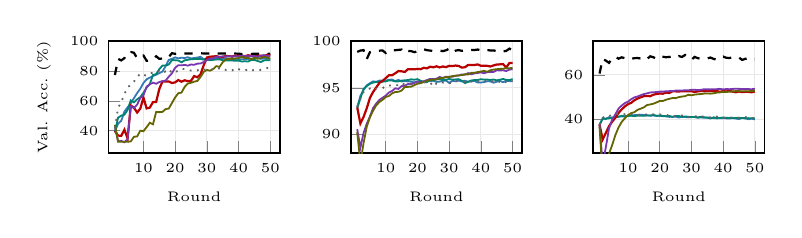
\begin{tikzpicture}
\begin{groupplot}[
  group style={
    xlabels at=edge bottom,
    ylabels at=edge left,
    group size=3 by 1,
    horizontal sep=0.9cm,
  },
  p1panel,
  width=0.31\textwidth,
]
\nextgroupplot[ymin=25, ymax=100,
  legend to name=legendPiid,
  legend style={legend columns=7, font=\tiny,
    /tikz/every even column/.append style={column sep=0.3em}}]
\addplot[black,thick,dashed] coordinates {
  (1,77.39) (2,88.20) (3,87.21) (4,88.74) (5,92.61) (6,92.88) (7,92.34) (8,88.65) (9,90.45) (10,90.54)
  (11,86.94) (12,87.21) (13,87.66) (14,90.00) (15,88.29) (16,88.47) (17,89.91) (18,89.55) (19,92.07) (20,91.62)
  (21,91.89) (22,91.89) (23,91.80) (24,91.80) (25,91.89) (26,91.98) (27,91.98) (28,91.98) (29,91.89) (30,91.89)
  (31,91.80) (32,91.89) (33,91.80) (34,91.80) (35,91.80) (36,91.80) (37,91.80) (38,91.71) (39,91.80) (40,91.71)
  (41,91.53) (42,91.71) (43,91.62) (44,91.53) (45,91.71) (46,91.71) (47,91.71) (48,91.62) (49,91.53) (50,91.71)};
\addlegendentry{Central}
\addplot[clBlue] coordinates {
  (1,39.59) (2,44.64) (3,46.67) (4,52.88) (5,55.68) (6,58.36) (7,61.84) (8,65.25) (9,68.14) (10,72.04)
  (11,74.51) (12,75.59) (13,76.74) (14,77.59) (15,78.68) (16,79.72) (17,83.36) (18,87.57) (19,88.26) (20,89.23)
  (21,88.63) (22,89.02) (23,88.80) (24,89.36) (25,88.48) (26,88.86) (27,89.12) (28,89.60) (29,88.05) (30,88.18)
  (31,88.39) (32,88.69) (33,88.76) (34,88.88) (35,88.27) (36,88.72) (37,88.05) (38,88.79) (39,87.76) (40,87.80)
  (41,88.05) (42,88.03) (43,88.13) (44,88.52) (45,88.07) (46,89.01) (47,88.23) (48,88.56) (49,88.25) (50,88.32)};
\addlegendentry{FedMD}
\addplot[clTeal] coordinates {
  (1,39.05) (2,48.77) (3,50.09) (4,50.77) (5,53.91) (6,60.36) (7,59.05) (8,61.05) (9,62.59) (10,65.48)
  (11,68.90) (12,71.33) (13,77.40) (14,78.05) (15,81.34) (16,83.70) (17,83.78) (18,84.49) (19,87.43) (20,87.36)
  (21,87.15) (22,85.92) (23,87.28) (24,87.60) (25,87.99) (26,88.11) (27,88.18) (28,88.13) (29,87.76) (30,87.54)
  (31,87.37) (32,87.58) (33,87.85) (34,87.89) (35,87.32) (36,87.16) (37,87.21) (38,87.16) (39,86.91) (40,87.08)
  (41,86.46) (42,86.65) (43,86.46) (44,87.43) (45,87.47) (46,86.83) (47,86.12) (48,87.21) (49,87.41) (50,87.24)};
\addlegendentry{FedAKD}
\addplot[clRed,thick] coordinates {
  (1,39.76) (2,36.73) (3,36.59) (4,40.64) (5,34.88) (6,56.95) (7,55.46) (8,52.23) (9,54.79) (10,62.27)
  (11,54.94) (12,55.50) (13,59.17) (14,59.30) (15,68.01) (16,73.11) (17,72.95) (18,73.03) (19,72.03) (20,72.47)
  (21,74.03) (22,72.93) (23,73.85) (24,73.26) (25,73.55) (26,76.71) (27,75.89) (28,77.80) (29,83.94) (30,89.14)
  (31,89.73) (32,89.80) (33,90.13) (34,89.39) (35,89.41) (36,90.27) (37,90.03) (38,89.86) (39,90.41) (40,90.35)
  (41,89.79) (42,89.93) (43,90.64) (44,90.32) (45,89.83) (46,90.33) (47,90.38) (48,89.94) (49,90.95) (50,90.32)};
\addlegendentry{FedMKS}
\addplot[clPurple] coordinates {
  (1,42.82) (2,32.87) (3,33.16) (4,32.24) (5,34.45) (6,56.31) (7,55.22) (8,57.55) (9,61.90) (10,63.79)
  (11,69.62) (12,71.14) (13,72.28) (14,71.52) (15,72.69) (16,73.23) (17,73.71) (18,76.29) (19,78.59) (20,82.28)
  (21,83.99) (22,83.90) (23,84.17) (24,83.71) (25,84.46) (26,84.24) (27,85.03) (28,85.12) (29,86.11) (30,87.30)
  (31,88.29) (32,88.48) (33,89.86) (34,89.59) (35,89.95) (36,89.80) (37,90.03) (38,90.05) (39,90.04) (40,90.01)
  (41,90.35) (42,90.30) (43,89.99) (44,90.16) (45,90.09) (46,89.71) (47,90.29) (48,90.80) (49,90.08) (50,90.47)};
\addlegendentry{FedAvg}
\addplot[clOlive] coordinates {
  (1,43.93) (2,32.61) (3,32.61) (4,32.61) (5,32.61) (6,32.78) (7,35.95) (8,36.13) (9,40.00) (10,39.65)
  (11,42.37) (12,45.33) (13,44.27) (14,52.55) (15,52.45) (16,52.66) (17,54.50) (18,54.88) (19,58.67) (20,62.37)
  (21,65.18) (22,65.59) (23,69.43) (24,71.68) (25,72.17) (26,72.95) (27,73.39) (28,76.08) (29,79.46) (30,80.80)
  (31,80.30) (32,81.43) (33,83.35) (34,82.83) (35,86.00) (36,87.87) (37,88.35) (38,88.11) (39,88.59) (40,88.77)
  (41,89.60) (42,88.78) (43,89.03) (44,87.94) (45,89.01) (46,88.38) (47,88.74) (48,89.53) (49,89.11) (50,88.47)};
\addlegendentry{FedProx}
\addplot[clGray,dotted] coordinates {
  (1,41.86) (2,55.45) (3,59.12) (4,64.68) (5,69.07) (6,70.86) (7,73.00) (8,75.77) (9,78.40) (10,77.35)
  (11,77.06) (12,77.95) (13,79.28) (14,79.12) (15,80.09) (16,78.73) (17,79.88) (18,78.53) (19,80.87) (20,79.61)
  (21,80.10) (22,81.52) (23,81.39) (24,80.87) (25,80.41) (26,80.64) (27,80.45) (28,81.85) (29,81.14) (30,81.22)
  (31,81.05) (32,81.15) (33,81.79) (34,81.86) (35,82.17) (36,80.77) (37,81.12) (38,80.50) (39,82.09) (40,81.31)
  (41,80.79) (42,80.42) (43,81.20) (44,80.19) (45,81.01) (46,80.84) (47,80.85) (48,81.38) (49,82.08) (50,81.78)};
\addlegendentry{Local}
\nextgroupplot[ymin=88, ymax=100,]
\addplot[black,thick,dashed] coordinates {
  (1,98.87) (2,99.01) (3,99.06) (4,98.08) (5,98.84) (6,98.95) (7,98.96) (8,99.0) (9,99.02) (10,98.75)
  (11,98.98) (12,99.06) (13,99.05) (14,99.08) (15,99.12) (16,98.74) (17,98.96) (18,98.95) (19,98.84) (20,98.92)
  (21,99.11) (22,99.15) (23,99.05) (24,99.01) (25,98.96) (26,98.98) (27,99.0) (28,98.95) (29,99.04) (30,99.2)
  (31,98.83) (32,99.0) (33,99.06) (34,98.98) (35,99.01) (36,99.01) (37,99.08) (38,99.07) (39,99.12) (40,99.03)
  (41,98.96) (42,99.07) (43,99.02) (44,99.03) (45,98.94) (46,99.03) (47,98.93) (48,98.97) (49,99.22) (50,99.04)};
\addplot[clBlue] coordinates {
  (1,92.94) (2,94.14) (3,94.76) (4,95.27) (5,95.5) (6,95.7) (7,95.66) (8,95.78) (9,95.78) (10,95.77)
  (11,95.88) (12,95.89) (13,95.73) (14,95.86) (15,95.69) (16,95.73) (17,95.69) (18,95.67) (19,95.59) (20,95.7)
  (21,95.66) (22,95.64) (23,95.75) (24,95.72) (25,95.78) (26,95.64) (27,95.67) (28,95.75) (29,95.79) (30,95.54)
  (31,95.75) (32,95.71) (33,95.78) (34,95.69) (35,95.77) (36,95.65) (37,95.72) (38,95.74) (39,95.58) (40,95.58)
  (41,95.62) (42,95.71) (43,95.7) (44,95.56) (45,95.66) (46,95.75) (47,95.61) (48,95.76) (49,95.73) (50,95.72)};
\addplot[clTeal] coordinates {
  (1,92.78) (2,93.88) (3,94.89) (4,95.2) (5,95.43) (6,95.57) (7,95.64) (8,95.62) (9,95.67) (10,95.7)
  (11,95.81) (12,95.79) (13,95.7) (14,95.7) (15,95.78) (16,95.82) (17,95.84) (18,95.92) (19,95.88) (20,95.94)
  (21,95.77) (22,95.65) (23,95.61) (24,95.91) (25,95.78) (26,95.97) (27,95.92) (28,95.85) (29,95.87) (30,95.97)
  (31,95.88) (32,95.91) (33,95.94) (34,95.76) (35,95.51) (36,95.66) (37,95.8) (38,95.85) (39,95.85) (40,95.93)
  (41,95.89) (42,95.9) (43,95.85) (44,95.9) (45,95.81) (46,95.88) (47,95.96) (48,95.86) (49,95.84) (50,95.95)};
\addplot[clRed,thick] coordinates {
  (1,92.9) (2,91.18) (3,91.88) (4,92.8) (5,93.92) (6,94.56) (7,95.05) (8,95.54) (9,95.75) (10,96.05)
  (11,96.36) (12,96.36) (13,96.57) (14,96.81) (15,96.78) (16,96.71) (17,97.01) (18,97.0) (19,96.99) (20,97.04)
  (21,97.01) (22,97.16) (23,97.1) (24,97.28) (25,97.21) (26,97.32) (27,97.2) (28,97.3) (29,97.23) (30,97.37)
  (31,97.34) (32,97.4) (33,97.36) (34,97.18) (35,97.22) (36,97.47) (37,97.45) (38,97.46) (39,97.52) (40,97.38)
  (41,97.37) (42,97.37) (43,97.3) (44,97.41) (45,97.51) (46,97.53) (47,97.56) (48,97.19) (49,97.67) (50,97.68)};
\addplot[clPurple] coordinates {
  (1,90.56) (2,88.58) (3,90.16) (4,91.14) (5,91.93) (6,92.83) (7,93.32) (8,93.71) (9,93.94) (10,94.17)
  (11,94.51) (12,94.67) (13,94.95) (14,94.89) (15,95.19) (16,95.24) (17,95.41) (18,95.39) (19,95.54) (20,95.66)
  (21,95.6) (22,95.72) (23,95.84) (24,95.96) (25,95.94) (26,95.98) (27,96.17) (28,96.06) (29,96.2) (30,96.2)
  (31,96.19) (32,96.3) (33,96.33) (34,96.44) (35,96.41) (36,96.59) (37,96.46) (38,96.56) (39,96.6) (40,96.67)
  (41,96.57) (42,96.69) (43,96.71) (44,96.71) (45,96.89) (46,96.87) (47,96.89) (48,96.81) (49,96.96) (50,97.01)};
\addplot[clOlive] coordinates {
  (1,90.24) (2,86.93) (3,89.07) (4,90.82) (5,91.85) (6,92.54) (7,93.13) (8,93.48) (9,93.72) (10,94.02)
  (11,94.13) (12,94.41) (13,94.56) (14,94.58) (15,94.71) (16,95.09) (17,95.11) (18,95.13) (19,95.29) (20,95.45)
  (21,95.5) (22,95.64) (23,95.77) (24,95.85) (25,95.92) (26,95.89) (27,96.05) (28,96.08) (29,96.15) (30,96.18)
  (31,96.26) (32,96.31) (33,96.34) (34,96.37) (35,96.47) (36,96.44) (37,96.63) (38,96.63) (39,96.7) (40,96.76)
  (41,96.83) (42,96.73) (43,96.89) (44,96.97) (45,97.01) (46,97.04) (47,97.05) (48,97.13) (49,97.1) (50,97.16)};
\addplot[clGray,dotted] coordinates {
  (1,92.99) (2,93.8) (3,94.54) (4,94.75) (5,94.94) (6,94.76) (7,94.93) (8,94.92) (9,94.96) (10,95.22)
  (11,95.25) (12,95.27) (13,95.34) (14,95.26) (15,95.51) (16,95.34) (17,95.31) (18,95.47) (19,95.49) (20,95.57)
  (21,95.5) (22,95.61) (23,95.54) (24,95.6) (25,95.15) (26,95.48) (27,95.66) (28,95.57) (29,95.49) (30,95.54)
  (31,95.52) (32,95.72) (33,95.7) (34,95.62) (35,95.64) (36,95.6) (37,95.68) (38,95.79) (39,95.72) (40,95.64)
  (41,95.77) (42,95.82) (43,95.81) (44,95.63) (45,95.77) (46,95.64) (47,95.47) (48,95.66) (49,95.74) (50,95.74)};

\nextgroupplot[ymin=25, ymax=75,]
\addplot[black,thick,dashed] coordinates {
  (1,60.59) (2,67.14) (3,66.37) (4,65.37) (5,67.36) (6,68.15) (7,67.25) (8,67.85) (9,67.46) (10,67.79)
  (11,67.15) (12,67.48) (13,67.52) (14,67.33) (15,66.5) (16,67.12) (17,68.3) (18,67.89) (19,67.18) (20,68.19)
  (21,68.09) (22,67.9) (23,68.02) (24,68.34) (25,67.83) (26,68.41) (27,68.02) (28,68.89) (29,67.64) (30,66.71)
  (31,68.04) (32,67.47) (33,67.19) (34,67.18) (35,67.36) (36,67.75) (37,67.14) (38,66.8) (39,67.71) (40,68.17)
  (41,67.63) (42,67.58) (43,67.81) (44,68.05) (45,67.74) (46,66.69) (47,67.2) (48,67.36) (49,66.86) (50,66.92)};
\addplot[clBlue] coordinates {
  (1,37.46) (2,40.5) (3,40.25) (4,41.06) (5,40.43) (6,41.41) (7,41.4) (8,41.34) (9,41.49) (10,41.7)
  (11,41.77) (12,41.98) (13,42.03) (14,42.18) (15,42.03) (16,41.91) (17,41.73) (18,41.79) (19,41.61) (20,41.71)
  (21,41.44) (22,41.44) (23,41.19) (24,41.24) (25,41.31) (26,40.9) (27,41.23) (28,41.13) (29,41.02) (30,41.07)
  (31,41.17) (32,40.82) (33,40.91) (34,40.83) (35,40.87) (36,40.83) (37,40.61) (38,40.53) (39,40.54) (40,40.59)
  (41,40.53) (42,40.46) (43,40.66) (44,40.44) (45,40.22) (46,40.72) (47,40.6) (48,40.13) (49,40.4) (50,40.04)};
\addplot[clTeal] coordinates {
  (1,37.54) (2,40.52) (3,40.38) (4,40.53) (5,40.96) (6,40.93) (7,41.21) (8,41.67) (9,41.34) (10,41.62)
  (11,41.74) (12,41.5) (13,41.74) (14,41.73) (15,41.68) (16,41.8) (17,41.79) (18,42.08) (19,41.69) (20,41.76)
  (21,41.63) (22,41.48) (23,41.62) (24,41.2) (25,41.55) (26,41.61) (27,41.14) (28,41.4) (29,41.22) (30,41.1)
  (31,41.11) (32,40.95) (33,41.24) (34,41.0) (35,40.85) (36,40.48) (37,41.0) (38,40.62) (39,40.72) (40,40.92)
  (41,40.76) (42,40.71) (43,40.65) (44,40.74) (45,40.61) (46,40.71) (47,40.48) (48,40.63) (49,40.56) (50,40.48)};
\addplot[clRed,thick] coordinates {
  (1,37.72) (2,31.11) (3,33.99) (4,37.04) (5,39.05) (6,40.85) (7,42.95) (8,44.56) (9,45.88) (10,46.91)
  (11,47.48) (12,48.62) (13,49.41) (14,49.95) (15,50.47) (16,50.59) (17,50.44) (18,51.13) (19,51.43) (20,51.65)
  (21,51.56) (22,52.08) (23,51.86) (24,52.63) (25,52.61) (26,52.53) (27,52.72) (28,52.61) (29,52.7) (30,52.63)
  (31,52.39) (32,52.58) (33,52.83) (34,52.7) (35,52.72) (36,52.86) (37,52.71) (38,52.76) (39,52.37) (40,52.74)
  (41,52.58) (42,52.86) (43,52.49) (44,52.23) (45,52.54) (46,52.27) (47,52.41) (48,52.38) (49,52.21) (50,52.57)};
\addplot[clPurple] coordinates {
  (1,37.85) (2,19.85) (3,27.68) (4,36.06) (5,39.99) (6,42.34) (7,44.9) (8,46.25) (9,47.37) (10,48.04)
  (11,49.12) (12,49.92) (13,50.33) (14,50.89) (15,51.39) (16,51.75) (17,52.1) (18,52.24) (19,52.28) (20,52.49)
  (21,52.51) (22,52.66) (23,52.71) (24,52.72) (25,52.96) (26,53.02) (27,52.98) (28,53.13) (29,53.07) (30,53.3)
  (31,53.34) (32,53.15) (33,53.31) (34,53.56) (35,53.5) (36,53.49) (37,53.6) (38,53.6) (39,53.74) (40,53.48)
  (41,53.66) (42,53.58) (43,53.7) (44,53.8) (45,53.72) (46,53.7) (47,53.67) (48,53.63) (49,53.56) (50,53.81)};
\addplot[clOlive] coordinates {
  (1,36.87) (2,14.87) (3,20.71) (4,24.74) (5,28.61) (6,33.05) (7,36.47) (8,38.94) (9,40.57) (10,41.98)
  (11,42.91) (12,43.28) (13,44.36) (14,44.88) (15,45.47) (16,46.5) (17,46.76) (18,47.09) (19,47.66) (20,48.33)
  (21,48.32) (22,48.87) (23,49.26) (24,49.63) (25,49.57) (26,50.03) (27,50.28) (28,50.47) (29,51.08) (30,50.85)
  (31,51.17) (32,51.32) (33,51.41) (34,51.62) (35,51.65) (36,51.6) (37,51.75) (38,52.05) (39,52.17) (40,52.38)
  (41,52.35) (42,52.46) (43,52.55) (44,52.76) (45,52.72) (46,52.62) (47,52.69) (48,52.67) (49,52.8) (50,52.93)};
\addplot[clGray,dotted] coordinates {
  (1,37.78) (2,40.77) (3,41.72) (4,41.52) (5,42.15) (6,42.33) (7,42.54) (8,42.59) (9,42.38) (10,42.43)
  (11,42.53) (12,42.49) (13,41.98) (14,42.3) (15,42.21) (16,42.28) (17,42.71) (18,42.3) (19,41.97) (20,42.32)
  (21,42.12) (22,42.19) (23,41.62) (24,41.61) (25,41.59) (26,41.84) (27,41.78) (28,41.91) (29,41.02) (30,41.46)
  (31,41.53) (32,41.27) (33,41.67) (34,41.1) (35,41.36) (36,40.88) (37,41.56) (38,41.3) (39,41.06) (40,40.71)
  (41,40.86) (42,40.84) (43,40.92) (44,40.97) (45,40.83) (46,41.19) (47,41.08) (48,40.91) (49,40.91) (50,40.53)};

\end{groupplot}
\end{tikzpicture}
\par\vspace{4pt}
\ref{legendPiid}
\caption{Validation accuracy over 50 rounds under IID partitioning
  (mean over completed seeds).  Panels: HomeOccupancy, MNIST, CIFAR-10.
  FedAvg/FedProx use the all-small architecture.  \dag~single-seed runs.}
\label{fig:mainiid}
\end{figure*}

\begin{figure*}[t]
\centering
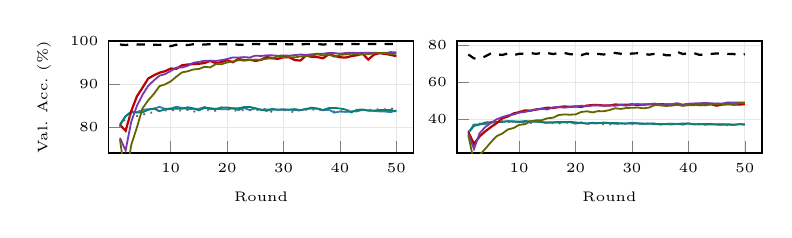
\begin{tikzpicture}
\begin{groupplot}[
  group style={
    xlabels at=edge bottom,
    ylabels at=edge left,
    group size=2 by 1,
    horizontal sep=0.55cm,
  },
  p1panel,
  width=0.45\textwidth,
]
\nextgroupplot[ymin=74, ymax=100,
  legend to name=legendPnoniid,
  legend style={legend columns=7, font=\tiny,
    /tikz/every even column/.append style={column sep=0.3em}}]
\addplot[black,thick,dashed] coordinates {
  (1,99.26) (2,99.15) (3,99.3) (4,99.27) (5,99.26) (6,99.31) (7,99.19) (8,99.18) (9,99.32) (10,98.88)
  (11,99.22) (12,99.32) (13,99.13) (14,99.33) (15,99.31) (16,99.26) (17,99.35) (18,99.31) (19,99.33) (20,99.31)
  (21,99.38) (22,99.2) (23,99.24) (24,99.39) (25,99.4) (26,99.32) (27,99.35) (28,99.4) (29,99.33) (30,99.39)
  (31,99.29) (32,99.38) (33,99.3) (34,99.37) (35,99.38) (36,99.41) (37,99.24) (38,99.41) (39,99.38) (40,99.31)
  (41,99.4) (42,99.4) (43,99.35) (44,99.38) (45,99.38) (46,99.4) (47,99.32) (48,99.41) (49,99.39) (50,99.38)};
\addplot[clBlue] coordinates {
  (1,80.44) (2,82.54) (3,83.49) (4,83.51) (5,84.04) (6,84.2) (7,84.29) (8,84.75) (9,84.28) (10,84.37)
  (11,84.76) (12,84.52) (13,84.21) (14,84.29) (15,84.29) (16,84.71) (17,84.26) (18,84.28) (19,84.22) (20,84.17)
  (21,84.42) (22,83.99) (23,84.49) (24,84.0) (25,84.44) (26,84.01) (27,84.13) (28,84.1) (29,84.13) (30,84.1)
  (31,84.09) (32,84.03) (33,83.96) (34,84.33) (35,84.35) (36,84.33) (37,83.94) (38,84.12) (39,83.4) (40,83.67)
  (41,83.57) (42,83.71) (43,83.71) (44,84.04) (45,83.96) (46,83.79) (47,83.7) (48,83.66) (49,83.53) (50,83.92)};
\addplot[clTeal] coordinates {
  (1,80.65) (2,82.6) (3,83.65) (4,83.43) (5,83.47) (6,84.07) (7,84.37) (8,83.77) (9,84.16) (10,84.27)
  (11,84.34) (12,84.3) (13,84.66) (14,84.4) (15,83.93) (16,84.52) (17,84.44) (18,84.27) (19,84.58) (20,84.62)
  (21,84.4) (22,84.41) (23,84.7) (24,84.75) (25,84.38) (26,84.12) (27,83.82) (28,84.28) (29,84.04) (30,84.17)
  (31,84.09) (32,84.23) (33,84.01) (34,84.19) (35,84.57) (36,84.37) (37,84.03) (38,84.47) (39,84.51) (40,84.37)
  (41,84.12) (42,83.46) (43,84.08) (44,84.13) (45,83.86) (46,83.9) (47,84.0) (48,84.01) (49,84.01) (50,83.67)};
\addplot[clRed,thick] coordinates {
  (1,80.55) (2,79.18) (3,83.77) (4,87.19) (5,89.22) (6,91.34) (7,92.09) (8,92.7) (9,93.05) (10,93.67)
  (11,93.62) (12,94.43) (13,94.61) (14,94.71) (15,94.78) (16,94.96) (17,95.45) (18,94.9) (19,95.17) (20,95.63)
  (21,95.13) (22,95.93) (23,95.59) (24,95.72) (25,95.45) (26,95.71) (27,96.37) (28,96.06) (29,95.93) (30,96.32)
  (31,96.3) (32,95.64) (33,95.53) (34,96.73) (35,96.35) (36,96.33) (37,96.07) (38,96.96) (39,96.63) (40,96.3)
  (41,96.22) (42,96.55) (43,96.76) (44,97.15) (45,95.75) (46,96.89) (47,97.24) (48,97.09) (49,96.84) (50,96.55)};
\addplot[clPurple] coordinates {
  (1,77.51) (2,74.6) (3,81.31) (4,84.98) (5,87.56) (6,89.62) (7,90.89) (8,92.01) (9,92.38) (10,93.11)
  (11,93.88) (12,93.9) (13,94.3) (14,95.01) (15,95.22) (16,95.49) (17,95.49) (18,95.44) (19,95.63) (20,95.89)
  (21,96.26) (22,96.23) (23,96.33) (24,96.24) (25,96.67) (26,96.6) (27,96.73) (28,96.74) (29,96.64) (30,96.73)
  (31,96.66) (32,96.8) (33,96.94) (34,96.86) (35,96.99) (36,97.12) (37,97.12) (38,97.29) (39,97.26) (40,97.13)
  (41,97.29) (42,97.36) (43,97.27) (44,97.36) (45,97.35) (46,97.34) (47,97.29) (48,97.24) (49,97.5) (50,97.41)};
\addplot[clOlive] coordinates {
  (1,77.16) (2,67.8) (3,75.88) (4,79.95) (5,84.41) (6,86.26) (7,87.74) (8,89.56) (9,89.99) (10,90.69)
  (11,91.78) (12,92.78) (13,93.03) (14,93.46) (15,93.58) (16,94.08) (17,93.94) (18,94.71) (19,94.68) (20,95.09)
  (21,95.3) (22,95.6) (23,95.56) (24,95.67) (25,95.75) (26,95.69) (27,95.96) (28,96.05) (29,96.53) (30,96.28)
  (31,96.31) (32,96.27) (33,96.49) (34,96.63) (35,96.64) (36,96.98) (37,96.7) (38,96.97) (39,96.43) (40,96.87)
  (41,96.95) (42,97.1) (43,97.05) (44,96.93) (45,97.02) (46,97.2) (47,97.28) (48,97.33) (49,97.02) (50,97.17)};
\addplot[clGray,dotted] coordinates {
  (1,80.01) (2,82.05) (3,82.82) (4,82.6) (5,82.89) (6,83.36) (7,83.44) (8,83.86) (9,83.93) (10,83.92)
  (11,84.07) (12,83.82) (13,84.03) (14,83.56) (15,84.13) (16,84.47) (17,83.77) (18,83.85) (19,84.64) (20,84.27)
  (21,83.81) (22,83.94) (23,83.97) (24,84.0) (25,83.89) (26,84.24) (27,84.27) (28,83.49) (29,84.04) (30,84.0)
  (31,83.85) (32,83.4) (33,84.12) (34,84.1) (35,84.05) (36,84.29) (37,83.78) (38,84.16) (39,83.66) (40,83.6)
  (41,84.03) (42,83.82) (43,83.67) (44,84.06) (45,84.11) (46,84.05) (47,84.24) (48,84.21) (49,84.36) (50,84.28)};

\nextgroupplot[ymin=22, ymax=82,]
\addplot[black,thick,dashed] coordinates {
  (1,74.92) (2,72.86) (3,72.67) (4,73.94) (5,75.54) (6,75.04) (7,74.7) (8,75.46) (9,74.63) (10,75.29)
  (11,75.46) (12,75.75) (13,75.28) (14,75.75) (15,75.75) (16,75.18) (17,75.73) (18,75.79) (19,75.09) (20,75.12)
  (21,74.58) (22,75.48) (23,74.83) (24,75.25) (25,74.93) (26,75.68) (27,75.75) (28,75.35) (29,74.78) (30,75.5)
  (31,75.57) (32,75.47) (33,74.84) (34,75.28) (35,75.39) (36,74.58) (37,74.45) (38,76.38) (39,75.2) (40,75.59)
  (41,75.65) (42,74.73) (43,75.06) (44,75.25) (45,75.49) (46,75.43) (47,75.28) (48,75.18) (49,74.65) (50,75.12)};
\addplot[clBlue] coordinates {
  (1,33.05) (2,37.32) (3,37.42) (4,37.58) (5,38.31) (6,38.53) (7,38.84) (8,39.15) (9,38.75) (10,38.97)
  (11,38.77) (12,38.88) (13,38.89) (14,38.54) (15,38.52) (16,38.54) (17,38.34) (18,38.6) (19,38.56) (20,37.87)
  (21,38.18) (22,37.86) (23,38.26) (24,38.12) (25,38.2) (26,38.1) (27,37.72) (28,37.91) (29,37.84) (30,38.31)
  (31,38.02) (32,37.7) (33,37.86) (34,37.8) (35,37.33) (36,37.5) (37,37.34) (38,37.62) (39,37.29) (40,38.03)
  (41,37.38) (42,37.63) (43,37.3) (44,37.35) (45,37.28) (46,37.27) (47,37.22) (48,37.08) (49,37.53) (50,37.17)};
\addplot[clTeal] coordinates {
  (1,32.9) (2,36.56) (3,37.34) (4,38.41) (5,38.63) (6,38.61) (7,38.74) (8,39.04) (9,39.13) (10,38.58)
  (11,39.19) (12,39.01) (13,38.95) (14,38.58) (15,38.22) (16,38.41) (17,38.71) (18,38.58) (19,38.77) (20,38.45)
  (21,38.18) (22,37.84) (23,38.07) (24,38.01) (25,38.36) (26,38.02) (27,38.18) (28,37.95) (29,37.87) (30,37.86)
  (31,37.83) (32,37.8) (33,37.75) (34,37.64) (35,37.53) (36,37.58) (37,37.78) (38,37.63) (39,37.86) (40,37.74)
  (41,37.48) (42,37.39) (43,37.62) (44,37.58) (45,37.39) (46,37.4) (47,37.5) (48,37.26) (49,37.45) (50,37.44)};
\addplot[clRed,thick] coordinates {
  (1,33.18) (2,26.86) (3,30.95) (4,33.67) (5,35.97) (6,38.0) (7,40.6) (8,41.65) (9,43.25) (10,43.98)
  (11,44.89) (12,44.76) (13,45.37) (14,45.83) (15,46.35) (16,46.21) (17,46.68) (18,47.05) (19,46.81) (20,47.07)
  (21,46.76) (22,47.49) (23,47.8) (24,47.77) (25,47.55) (26,47.5) (27,48.06) (28,47.95) (29,47.89) (30,48.18)
  (31,47.8) (32,48.12) (33,48.15) (34,48.22) (35,48.2) (36,48.14) (37,48.07) (38,48.26) (39,47.64) (40,48.25)
  (41,48.04) (42,47.8) (43,47.78) (44,48.29) (45,47.44) (46,48.05) (47,48.2) (48,48.12) (49,48.0) (50,48.29)};
\addplot[clPurple] coordinates {
  (1,32.12) (2,24.2) (3,32.69) (4,35.99) (5,38.17) (6,40.09) (7,41.32) (8,42.24) (9,42.66) (10,43.72)
  (11,44.08) (12,44.77) (13,45.44) (14,45.77) (15,45.42) (16,46.52) (17,46.73) (18,46.37) (19,46.69) (20,46.99)
  (21,47.42) (22,47.17) (23,47.51) (24,47.62) (25,47.35) (26,47.71) (27,47.35) (28,47.86) (29,47.44) (30,47.97)
  (31,48.35) (32,47.81) (33,48.24) (34,48.6) (35,48.0) (36,48.22) (37,48.16) (38,48.8) (39,48.0) (40,48.49)
  (41,48.65) (42,48.76) (43,48.9) (44,48.75) (45,48.56) (46,48.58) (47,49.21) (48,49.14) (49,49.21) (50,49.07)};
\addplot[clOlive] coordinates {
  (1,31.52) (2,17.03) (3,20.91) (4,24.3) (5,27.84) (6,31.04) (7,32.45) (8,34.67) (9,35.43) (10,37.13)
  (11,37.47) (12,38.98) (13,39.58) (14,39.65) (15,40.67) (16,40.96) (17,42.42) (18,42.75) (19,42.59) (20,42.75)
  (21,44.06) (22,44.43) (23,43.85) (24,44.52) (25,44.46) (26,45.07) (27,46.05) (28,45.71) (29,46.17) (30,46.34)
  (31,46.43) (32,46.05) (33,46.41) (34,47.7) (35,47.62) (36,47.29) (37,47.44) (38,47.92) (39,47.36) (40,47.71)
  (41,47.68) (42,48.07) (43,47.67) (44,48.17) (45,48.48) (46,48.34) (47,48.39) (48,47.95) (49,48.77) (50,48.89)};
\addplot[clGray,dotted] coordinates {
  (1,33.25) (2,37.44) (3,37.83) (4,38.39) (5,38.63) (6,38.51) (7,39.13) (8,38.61) (9,38.84) (10,38.25)
  (11,38.02) (12,38.1) (13,38.85) (14,38.71) (15,37.91) (16,37.97) (17,37.86) (18,38.26) (19,38.37) (20,37.77)
  (21,38.53) (22,37.58) (23,37.98) (24,37.85) (25,37.4) (26,37.37) (27,37.65) (28,37.67) (29,37.84) (30,37.53)
  (31,37.5) (32,37.93) (33,37.81) (34,37.89) (35,37.47) (36,37.79) (37,37.78) (38,37.49) (39,37.29) (40,37.49)
  (41,37.46) (42,37.8) (43,37.22) (44,37.59) (45,37.59) (46,37.1) (47,36.97) (48,36.98) (49,37.91) (50,37.3)};

\end{groupplot}
\end{tikzpicture}
\par\vspace{4pt}
\ref{legendPnoniid}
\caption{Validation accuracy under non-IID partitioning
  (Dirichlet $\alpha{=}0.5$).  Panels: MNIST, CIFAR-10 (HomeOccupancy
  non-IID runs in progress).}
\label{fig:mainnoniid}
\end{figure*}

\textbf{HomeOccupancy.}
Under IID, FedMKS (90.4\%) and FedAvg (89.5\%) approach the centralised
ceiling (90.8\%), while FedMD (88.5\%) and FedAKD (87.0\%) lag without
weight sharing; Local plateaus at 80.4\%.  Under non-IID, completed
weight-sharing runs (FedAvg 38.4\%, FedProx 33.7\%) already trail
local-only training (60.1\%).

\textbf{MNIST.}
IID: Central 99.0\%, FedMKS 97.7\%, FedAvg/FedProx 97.0\%/97.2\%,
FedMD/FedAKD/Local ${\approx}95.8\%$.  Non-IID: FedAvg 97.4\%, FedProx
97.2\%, FedMKS 96.6\%, while FedMD/FedAKD/Local plateau at
${\approx}84\%$---${\approx}13$ points below the all-small weight-sharing
methods despite their larger architectures.

\textbf{CIFAR-10.}
Cross-domain public data (MNIST) gives little signal: all FL methods fall
$10$--$30\%$ below centralised.  FedAvg (53.8\%) edges FedProx (52.9\%)
and FedMKS (52.6\%) under IID, and leads under non-IID (49.1\% vs.\
48.9\%/48.3\%).  KD-only methods (FedMD 37.2\%, FedAKD 37.4\%) do not
beat Local (37.3\%).

\paragraph{Key observation.}
Under non-IID, weight sharing beats cross-architecture distillation even
when weight sharers are forced onto the smallest model (MNIST:
${\approx}97\%$ vs.\ ${\approx}84\%$).  FedMKS is designed to recover
model-sharing accuracy while preserving the heterogeneity that only
distillation permits.

\subsubsection{Ablation Studies}

\paragraph{Tier heterogeneity.}
Fig.~\ref{fig:tierablation} ablates the tier distribution for FedMD on
HomeOccupancy.  Under IID all configurations converge to
${\approx}86\%$; under non-IID \texttt{uniform} (61.5\%) beats
\texttt{all\_small} (59.1\%) and \texttt{skewed} (58.6\%)---small-dominated
tiers underperform a balanced mix under label skew.

\begin{figure*}[t]
\centering
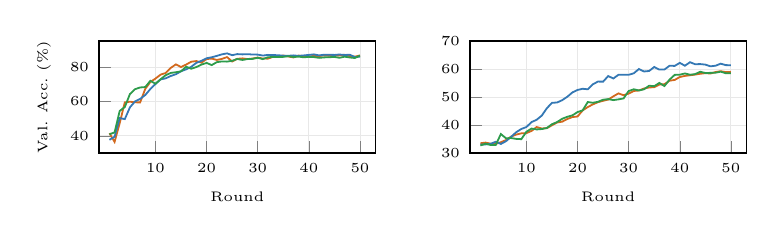
\begin{tikzpicture}
\begin{groupplot}[
  group style={
    xlabels at=edge bottom,
    ylabels at=edge left,
    group size=2 by 1,
    horizontal sep=1.2cm,
  },
  p1panel,
  width=0.42\textwidth,
]
\nextgroupplot[ymin=30, ymax=95,
  legend to name=legendPtwo,
  legend style={legend columns=3, font=\tiny}]
\addplot[clOrange] coordinates {
  (1,41.55) (2,36.48) (3,47.35) (4,59.50) (5,59.88) (6,59.51) (7,59.48) (8,67.32) (9,71.36) (10,73.32)
  (11,75.65) (12,76.59) (13,79.61) (14,81.60) (15,80.04) (16,81.49) (17,83.15) (18,83.54) (19,82.60) (20,84.71)
  (21,84.96) (22,84.17) (23,84.80) (24,85.84) (25,83.27) (26,84.85) (27,85.09) (28,84.69) (29,84.98) (30,85.56)
  (31,84.99) (32,84.95) (33,85.99) (34,86.03) (35,86.77) (36,86.20) (37,85.62) (38,86.71) (39,86.37) (40,86.12)
  (41,86.56) (42,86.44) (43,86.87) (44,86.65) (45,86.82) (46,86.84) (47,87.21) (48,86.39) (49,86.08) (50,86.84)};
\addlegendentry{All-Small}
\addplot[clBlue] coordinates {
  (1,37.71) (2,39.48) (3,50.34) (4,49.75) (5,56.57) (6,60.07) (7,61.51) (8,63.75) (9,67.26) (10,70.17)
  (11,72.85) (12,73.48) (13,74.86) (14,75.87) (15,77.59) (16,78.70) (17,80.21) (18,82.48) (19,83.68) (20,85.14)
  (21,85.74) (22,86.55) (23,87.44) (24,88.00) (25,86.96) (26,87.58) (27,87.42) (28,87.55) (29,87.33) (30,87.28)
  (31,86.73) (32,87.12) (33,87.01) (34,86.94) (35,86.63) (36,86.60) (37,86.83) (38,86.53) (39,86.82) (40,87.11)
  (41,87.42) (42,86.82) (43,87.23) (44,87.18) (45,87.11) (46,87.34) (47,87.06) (48,87.22) (49,85.86) (50,86.09)};
\addlegendentry{Uniform}
\addplot[clGreen] coordinates {
  (1,40.93) (2,41.99) (3,54.49) (4,56.77) (5,64.31) (6,67.15) (7,68.17) (8,68.40) (9,72.03) (10,70.36)
  (11,72.94) (12,75.31) (13,76.63) (14,77.03) (15,77.57) (16,80.23) (17,79.05) (18,80.05) (19,81.46) (20,82.45)
  (21,81.19) (22,82.89) (23,83.31) (24,83.21) (25,83.69) (26,84.74) (27,84.18) (28,84.68) (29,84.82) (30,85.44)
  (31,84.67) (32,85.75) (33,85.90) (34,85.95) (35,85.97) (36,86.37) (37,85.88) (38,86.14) (39,85.70) (40,85.99)
  (41,85.84) (42,85.40) (43,85.67) (44,85.77) (45,85.94) (46,85.44) (47,86.09) (48,85.61) (49,85.31) (50,86.70)};
\addlegendentry{Skewed}
\nextgroupplot[ymin=30, ymax=70,]
\addplot[clOrange] coordinates {
  (1,33.51) (2,33.74) (3,33.36) (4,33.27) (5,33.89) (6,34.64) (7,35.89) (8,36.61) (9,37.05) (10,37.14)
  (11,37.92) (12,39.31) (13,38.79) (14,38.91) (15,39.94) (16,40.94) (17,41.24) (18,42.18) (19,42.89) (20,43.09)
  (21,45.26) (22,46.47) (23,47.43) (24,48.21) (25,48.71) (26,49.14) (27,50.30) (28,51.36) (29,50.72) (30,51.28)
  (31,52.23) (32,52.40) (33,53.11) (34,53.48) (35,53.59) (36,54.51) (37,54.67) (38,55.91) (39,56.18) (40,57.23)
  (41,57.62) (42,57.86) (43,58.09) (44,58.40) (45,58.61) (46,58.48) (47,59.01) (48,59.31) (49,58.99) (50,59.07)};
\addplot[clBlue] coordinates {
  (1,33.02) (2,33.09) (3,33.31) (4,34.05) (5,33.25) (6,34.24) (7,35.80) (8,37.46) (9,38.62) (10,39.32)
  (11,41.09) (12,41.91) (13,43.41) (14,46.05) (15,47.99) (16,48.10) (17,48.93) (18,50.16) (19,51.72) (20,52.59)
  (21,53.02) (22,52.83) (23,54.64) (24,55.59) (25,55.57) (26,57.58) (27,56.70) (28,58.02) (29,58.03) (30,58.02)
  (31,58.56) (32,60.09) (33,59.21) (34,59.39) (35,60.82) (36,59.89) (37,59.91) (38,61.27) (39,61.21) (40,62.30)
  (41,61.27) (42,62.53) (43,61.81) (44,61.86) (45,61.67) (46,61.06) (47,61.28) (48,62.01) (49,61.49) (50,61.45)};
\addplot[clGreen] coordinates {
  (1,32.70) (2,33.35) (3,32.86) (4,32.88) (5,36.81) (6,35.29) (7,35.37) (8,35.07) (9,34.97) (10,37.63)
  (11,38.77) (12,38.45) (13,38.59) (14,38.99) (15,40.32) (16,41.10) (17,42.28) (18,42.98) (19,43.50) (20,44.68)
  (21,45.29) (22,48.26) (23,48.01) (24,48.35) (25,49.10) (26,49.32) (27,48.96) (28,49.22) (29,49.56) (30,52.21)
  (31,52.84) (32,52.42) (33,52.82) (34,54.11) (35,53.95) (36,55.11) (37,53.99) (38,56.31) (39,57.99) (40,58.06)
  (41,58.50) (42,58.05) (43,58.27) (44,59.10) (45,58.67) (46,58.71) (47,58.77) (48,59.14) (49,58.58) (50,58.57)};
\end{groupplot}
\end{tikzpicture}
\par\vspace{4pt}
\ref{legendPtwo}
\caption{FedMD tier-heterogeneity ablation on HomeOccupancy, IID (left)
  and non-IID (right): \texttt{all\_small} (100\%~S), \texttt{uniform}
  (35/35/30), \texttt{skewed} (60/30/10).}
\label{fig:tierablation}
\end{figure*}

\paragraph{FedMKS vs.\ FedDF.}
Fig.~\ref{fig:feddf} and Table~\ref{tab:efficiency} compare FedMKS and
FedDF on HomeOccupancy (IID, single seed, 30 rounds, 10 clients).  FedDF
converges faster (plateau near round~10, 89.0\% vs.\ 87.1\% final-five
mean), though FedMKS is still climbing and edges ahead at round~30
(88.2\% vs.\ 88.1\%).  The efficiency profiles differ sharply: FedDF
spends ${\approx}243$~s/round on server-side ensemble training, whereas
FedMKS does essentially no server compute (${\approx}0.06$~s) and
distributes distillation across parallel clients (${\approx}93$~s vs.\
${\approx}25$~s per client).  FedMKS removes the serial server bottleneck
at ${\approx}22\%$ higher communication (37.9 vs.\ 31.0~MB/round); the whole ${\approx}6.9$~MB overhead is the soft-label exchange
($|\mathcal{D}^{\text{pub}}|{\times}d$ each way), which FedDF avoids by
distilling on the server.  The dashed curve in Fig.~\ref{fig:feddf} shows
FedMKS with Mixup disabled on the public set: convergence is comparable
and the final accuracy drops only ${\approx}1$~pp (87.3\% vs.\ 88.2\% at
round~30), indicating that Mixup yields a modest regularisation benefit
rather than being essential to the hybrid update.

\begin{figure}[t]
\centering
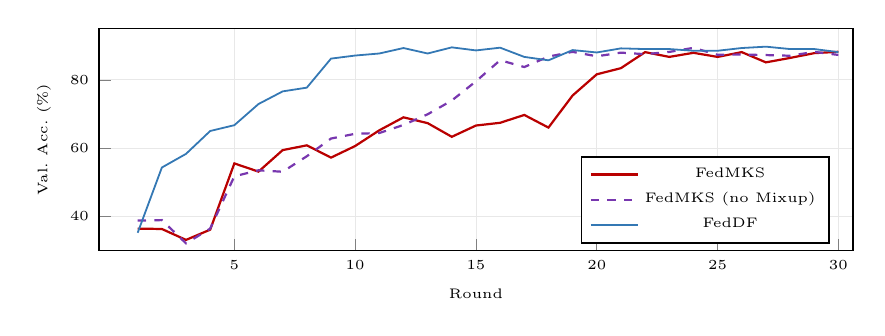
\begin{tikzpicture}
\begin{axis}[p1panel, width=0.92\columnwidth, height=4.4cm,
  xmin=0, xmax=30, ymin=30, ymax=95, xtick={5,10,15,20,25,30},
  legend pos=south east, legend style={font=\tiny}]
\addplot[clRed,thick,mark=none] coordinates {
  (1,36.4) (2,36.3) (3,33.1) (4,36.1) (5,55.5) (6,53.1) (7,59.4) (8,60.8)
  (9,57.2) (10,60.6) (11,65.2) (12,69.0) (13,67.3) (14,63.3) (15,66.6)
  (16,67.4) (17,69.7) (18,66.0) (19,75.4) (20,81.6) (21,83.4) (22,88.1)
  (23,86.7) (24,87.9) (25,86.7) (26,88.1) (27,85.1) (28,86.4) (29,87.8)
  (30,88.2)};
\addlegendentry{FedMKS}
\addplot[clPurple,thick,dashed,mark=none] coordinates {
  (1,38.77) (2,38.90) (3,32.09) (4,36.40) (5,51.73) (6,53.48) (7,53.06)
  (8,57.60) (9,62.79) (10,64.18) (11,64.40) (12,66.78) (13,69.89)
  (14,73.93) (15,79.55) (16,85.73) (17,83.73) (18,86.79) (19,88.18)
  (20,86.88) (21,87.95) (22,87.50) (23,88.16) (24,89.35) (25,87.32)
  (26,87.39) (27,87.24) (28,87.04) (29,88.18) (30,87.28)};
\addlegendentry{FedMKS (no Mixup)}
\addplot[clBlue,mark=none] coordinates {
  (1,35.2) (2,54.3) (3,58.3) (4,65.0) (5,66.7) (6,72.9) (7,76.6) (8,77.7)
  (9,86.2) (10,87.1) (11,87.7) (12,89.3) (13,87.7) (14,89.5) (15,88.6)
  (16,89.4) (17,86.7) (18,85.7) (19,88.7) (20,88.0) (21,89.2) (22,89.0)
  (23,89.0) (24,88.5) (25,88.5) (26,89.3) (27,89.7) (28,89.0) (29,89.0)
  (30,88.1)};
\addlegendentry{FedDF}
\end{axis}
\end{tikzpicture}
\caption{FedMKS vs.\ FedDF validation accuracy on HomeOccupancy
  (IID, 30 rounds, 10 clients). The dashed curve is a FedMKS ablation
  with Mixup augmentation on the public set disabled.}
\label{fig:feddf}
\end{figure}

\begin{figure}[t]
\centering
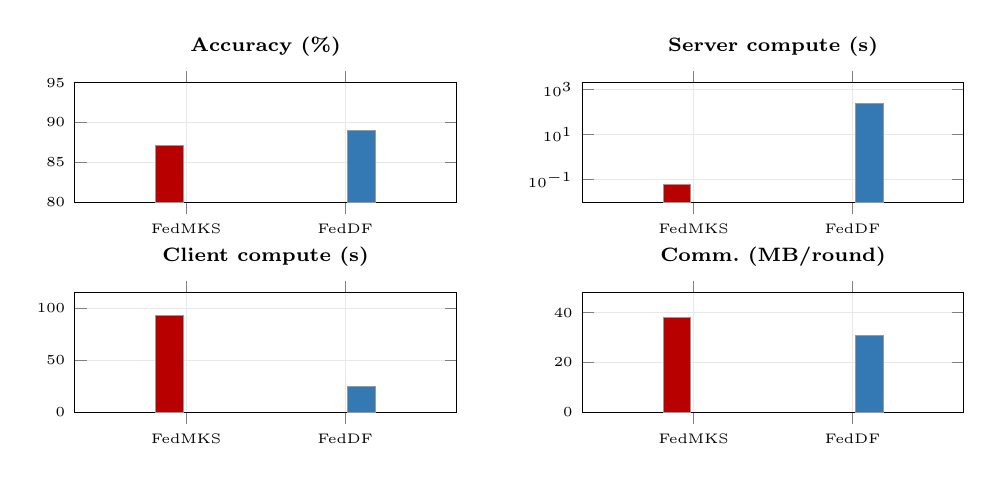
\begin{tikzpicture}
\begin{groupplot}[
  group style={group size=2 by 2,
    horizontal sep=1.6cm, vertical sep=1.15cm},
  width=0.53\columnwidth, height=3.1cm,
  xtick={1,2}, xticklabels={FedMKS,FedDF}, xmin=0.3, xmax=2.7,
  tick label style={font=\tiny}, label style={font=\tiny},
  title style={font=\scriptsize\bfseries},
  grid=major, grid style={gray!18, line width=0.3pt},
  every axis plot/.append style={draw=black!40},
]
\nextgroupplot[ybar, title={Accuracy (\%)}, ymin=80, ymax=95]
\addplot[fill=clRed]  coordinates {(1,87.1)};
\addplot[fill=clBlue] coordinates {(2,89.0)};
\nextgroupplot[ybar, title={Server compute (s)}, ymode=log,
  ymin=0.01, ymax=2000, log origin=infty]
\addplot[fill=clRed]  coordinates {(1,0.06)};
\addplot[fill=clBlue] coordinates {(2,243.2)};
\nextgroupplot[ybar, title={Client compute (s)}, ymin=0, ymax=115]
\addplot[fill=clRed]  coordinates {(1,93.1)};
\addplot[fill=clBlue] coordinates {(2,24.6)};
\nextgroupplot[ybar, title={Comm.\ (MB/round)}, ymin=0, ymax=48]
\addplot[fill=clRed]  coordinates {(1,37.9)};
\addplot[fill=clBlue] coordinates {(2,31.0)};
\end{groupplot}
\end{tikzpicture}
\caption{Compute, communication, and accuracy comparison of FedMKS and
  FedDF on HomeOccupancy (cf.\ Table~\ref{tab:efficiency}).  FedMKS
  eliminates the server bottleneck at ${\approx}22\%$ higher
  communication and higher per-client compute.}
\label{fig:efficiency}
\end{figure}

\begin{table}[t]
\centering\small
\caption{Efficiency comparison on HomeOccupancy (per round unless
  noted; accuracy = final-five-round mean).}
\label{tab:efficiency}
\setlength{\tabcolsep}{5pt}
\begin{tabular}{@{}lcc@{}}
\toprule
\textbf{Metric (per round)} & \textbf{FedMKS} & \textbf{FedDF}\\
\midrule
Final val.\ accuracy (\%)        & 87.1   & 89.0  \\
Server compute (s)               & 0.06   & 243.2 \\
Mean client compute (s)          & 93.1   & 24.6  \\
\midrule
Comm.: model weights (MB)        & 31.0   & 31.0  \\
Comm.: soft labels (MB)          & 6.9    & 0.0   \\
Communication total (MB)         & 37.9   & 31.0  \\
\midrule
Total communication (MB, 30 r.)  & 1137.7 & 930.1 \\
\bottomrule
\end{tabular}
\end{table}

% ─────────────────────────────────────────────────────────────────────────────
\section{Conclusion}
\label{sec:conclusion}

We presented \textbf{FedMKS}, a heterogeneous federated
knowledge-distillation algorithm for CSI-based indoor sensing that couples
intra-tier weight sharing with cross-tier soft-label distillation.  FedMKS
reaches near-centralised accuracy on HomeOccupancy
($\Delta{\approx}0.5\%$ under IID) while preserving architectural
heterogeneity, and matches FedDF accuracy (87.1\% vs.\ 89.0\%) while
eliminating its ${\approx}243$~s/round server bottleneck
(${\approx}0.06$~s/round) at ${\approx}22\%$ higher communication.

% ─────────────────────────────────────────────────────────────────────────────
\section{Limitations and Future Work}
\label{sec:limitations}

The main comparison uses a single uniform tier distribution; FedMKS also incurs
higher communication than FedMD, motivating weight compression
(quantisation, top-$k$).  Cross-domain public data gave little signal on
CIFAR-10, so domain-adapted or synthetic public sets remain open.
Finally, HomeSenseKD assumes synchronous rounds; asynchronous aggregation
under dropouts is an important extension.

% ─────────────────────────────────────────────────────────────────────────────
\section*{Code and Data Availability}

Source code is available at
\url{https://github.com/gadm21/HomeSenseKD}.
HomeOccupancy and HomeHAR datasets are hosted on HuggingFace at
\url{https://huggingface.co/gadgadgad}.

% ─────────────────────────────────────────────────────────────────────────────
\bibliographystyle{IEEEtran}
\bibliography{references}

\end{document}
